\documentclass[conference]{IEEEtran}
\usepackage{cite}
\usepackage{amsmath,amssymb,amsfonts}
\usepackage{xcolor}
\definecolor{nscblue}{RGB}{16,63,120}
\definecolor{nscteal}{RGB}{0,102,102}
\definecolor{nscpurple}{RGB}{106,40,120}
\usepackage{booktabs}
\usepackage{url}
\usepackage{graphicx}
\usepackage{tikz}
\usetikzlibrary{shapes.geometric,arrows.meta,positioning,fit}

\def\BibTeX{{\rm B\kern-.05em{\sc i\kern-.025em b}\kern-.08em
    T\kern-.1667em\lower.7ex\hbox{E}\kern-.125emX}}

\begin{document}

\title{Fast, Error-Resilient Intent Recognition for Offline Security Copilots: A Guarded LLM Pipeline}

\author{\IEEEauthorblockN{P.~M.~T.~L.~Karunarathna}
\IEEEauthorblockA{\textit{Department of Computer System Engineering}\\
\textit{Sri Lanka Institute of Information Technology}\\
Malabe, Sri Lanka\\
it22249852@my.sliit.lk}}

\maketitle

\begin{abstract}
Large language models (LLMs) are increasingly proposed as copilots for penetration testing and defensive security operations. However, LLMs hallucinate fabricated CVEs, malformed commands, and parameter values, and they can be diverted by adversarial prompt engineering, which makes their output unusable in operational security tooling. This paper presents a guarded, retrieval-free intent-recognition engine that wraps an offline, CPU-only attacker-guided LLM (Qwen or Gemma; exact model tags in Section~\ref{sec:method}) with a seven-stage normalizing pipeline, three-layer adversarial detection, role-based access control, deterministic schema and network validation, and a semantic self-consistency gate. We contribute a purpose-built 900-record data set (400 well-formed and 500 flawed prompts across eight categories) and an ablation methodology that isolates each defense layer. Across four experiments on a single consumer laptop, the guarded pipeline raises intent-recognition accuracy from 69--78\% to 82--86\%, raises flaw-catch rate from $0\%$ to 72\% (Gemma) and 64\% (Qwen) on the stratified holdout and to 84\% on the 900-record ablation set, and cuts false positives from 31--32\% to 14--15\%; the largest single layer (hallucination validation) contributes up to 22 points of catch rate. All measurements are single-run point estimates from one backend pass per configuration, without confidence intervals or seed sweeps; the resulting uncertainty is discussed in the Limitations section. We discuss failure modes unique to offline LLM backends and analyze the residual threats.
\end{abstract}

\begin{IEEEkeywords}
intent recognition, LLM guardrails, hallucination detection, prompt injection, RBAC
\end{IEEEkeywords}

\section{INTRODUCTION}
Security operations today are bottlenecked by expertise. Penetration testers, security analysts, and blue teams must map free-form intent onto tools, commands, and targets while complying with authorization boundaries. Recent work has shown that large language models (LLMs) can act as \emph{AI sparring partners} for this work, producing realistic attack plans and even executing exploitation steps in controlled environments~\cite{deng2024pentestgpt,happe2023pwned}. Demonstrations of indirect prompt injection and dual-use abuse, however, show that the same model that helps a defender can be hijacked by a user or by text retrieved from a web page~\cite{greshake2023indirect,liu2023promptinjection,kang2024dualuse}.

An intent-recognition engine sits between the operator and the security toolchain: it classifies what the operator wants --- run a port scan, check a CVE, brute-force a password --- and emits a machine-consumable structure. If that engine is powered by an LLM, three classes of failure emerge. First, \emph{hallucination}: the model fabricates a CVE identifier, a parameter, or a claim, and the downstream tool acts on non-existent data~\cite{ji2023hallucination,farquhar2024semantic}. Second, \emph{adversarial deflection}: a prompt is worded so that the model abandons the classification task and emits attacker-chosen text~\cite{liu2023promptinjection,greshake2023indirect}. Third, \emph{authorization leakage}: unrestricted models answer out-of-policy request categories (exploitation, password attacks) for users who lack permission.

This paper addresses the question: \emph{can a small, offline, unattended LLM be made reliable enough to drive an operational security copilot?} We answer with NeuroShell IRE (\emph{Intent Recognition Engine}), a guarded pipeline in which a 7~B-parameter model is treated as an unreliable \emph{proposition generator} whose output is validated deterministically. The architecture (Section~\ref{sec:arch}) combines schema and regex validation, a network validator that checks targets against authorization policy, a scope guard, a three-layer adversarial detector, role-based access control (RBAC), a semantic cache, and a self-consistency gate built on semantic-clustering agreement. Four experiments (Section~\ref{sec:results}) on a consumer laptop without a GPU measure accuracy, flaw catch, and ablation impact of every layer, and identify the largest contributors to safety. The dataset and evaluation harness are versioned with the project source and reproducible from a single evaluation manifest.

The contributions of this work are: (i) a seven-stage, five-middleware architecture (S6B is the network sub-validator of S6) that subjects an offline LLM's output to deterministic, auditable validation before use; (ii) a purpose-built 900-record data set spanning eight flaw categories; (iii) a per-layer ablation methodology and results quantifying each defense's contribution; and (iv) a quantitative comparison of two LLM backends (Gemma and Qwen) under the same guardrail stack.

\section{RELATED WORK}
\textbf{LLMs for security tooling.} Happe and Cito~\cite{happe2023pwned} proposed LLMs as sparring partners for penetration testing and demonstrated a closed-loop system that drove a vulnerable virtual machine to root. Deng \emph{et al.}~\cite{deng2024pentestgpt} built PENTESTGPT, an LLM-centric assistant that decomposes penetration-testing tasks across a reasoning, generation, and guidance chain. Both works focus on the \emph{generation} side --- producing plausible next actions --- and treat output correctness informally; neither validates or authorizes the output before execution.

\textbf{Attacks on LLM-integrated applications.} Greshake \emph{et al.}~\cite{greshake2023indirect} introduced indirect prompt injection, where an attacker plants instructions in data that the model later ingests, and demonstrated compromise of real-world systems. Liu \emph{et al.}~\cite{liu2023promptinjection} formalized prompt-injection attacks and systematically benchmarked ten defenses, finding that prevention-based defenses were weak and detection-based defenses incomplete. Kang \emph{et al.}~\cite{kang2024dualuse} showed that dual-use attacks inspired by classic computer security bypass in-the-wild LLM content defenses with near-perfect success. The OWASP Top~10 for LLM Applications~\cite{owasp2025} formally catalogues these risks --- prompt injection (LLM01), sensitive-information disclosure (LLM02), and others --- as first-class application concerns.

\textbf{Hallucination detection.} \emph{Ji et al.}~\cite{ji2023hallucination} survey hallucination across natural-language generation, distinguishing intrinsic from extrinsic hallucination. Sampling-based methods detect failures without external knowledge: Manakul \emph{et al.}~\cite{manakul2023selfcheckgpt} proposed SelfCheckGPT, which scores the consistency of sampled responses; Kuhn \emph{et al.}~\cite{kuhn2023semantic} framed answer agreement via semantic uncertainty, and Farquhar \emph{et al.}~\cite{farquhar2024semantic} used semantic entropy over meaning clusters to detect confabulations in free-form text. These methods assume interactive or repeated generation; our contribution applies the disagreement intuition to a \emph{single} guarded classification with a hard latency budget, which we argue is the more realistic constraint in tool-in-the-loop security products.

\textbf{Retrieval and embeddings.} Retrieval-augmented generation (RAG)~\cite{lewis2020rag} grounds answers in external corpora, and sentence-level embeddings trained with bi-encoders (Sentence-BERT)~\cite{reimers2019sbert} provide the semantic distance signals used by our self-consistency gate and semantic cache. Unlike RAG, NeuroShell IRE deliberately performs no retrieval at inference time, keeping the offline, single-device deployment boundary free of new attack surface (retrieved data is itself a prompt-injection vector~\cite{greshake2023indirect}).

\section{RESEARCH GAP}
Two gaps motivate this work. First, the LLM-security copilot systems examined above validate their output informally, if at all: outputs are plausible prose consumed by humans. When a copilot's output is fed to an \emph{automated} toolchain --- the natural integration point for intent recognition --- hallucinated CVEs, malformed JSON, and injected text become machine-dispatched actions, not display text. The failure semantics change and the defense requirement becomes correctness, not plausibility. Second, the security literature evaluates defenses on cloud-hosted models with interactive budgets; we are not aware of prior work reporting a quantitative, per-layer ablation of a guardrail stack for a \emph{small offline} model running unattended in the field, where a retry loop or a verifier LLM doubles a multi-second CPU inference cost. We therefore ask three concrete research questions:

\begin{itemize}
\item \textbf{RQ1} How much does a stacked validation pipeline improve structured intent-recognition accuracy and flaw catching over raw LLM output?
\item \textbf{RQ2} Which individual guardrail layer contributes the most to catch rate, and which layers interact destructively?
\item \textbf{RQ3} Do the guardrails generalize across two different offline LLM backends?
\end{itemize}

\section{RESEARCH OBJECTIVES}
To answer the research questions we pursue four objectives:

\begin{enumerate}
\item Build a guarded intent-recognition engine that consumes free-text security requests and emits strictly-schema-validated, authorized intent structures with an average end-to-end latency compatible with single-user offline use.
\item Construct a 900-record data set covering 400 well-formed prompts and 500 deliberately flawed prompts across eight flaw categories (adversarial injection, out-of-scope, ambiguous, contradictory, fabricated parameter, fabricated CVE, type mismatch, and RBAC violation).
\item Establish an ablation protocol in which each guardrail is independently disabled while all others remain active, enabling an honest causal estimate of each layer's contribution.
\item Compare two offline LLM backends (Gemma and Qwen) under the identical guardrail stack to measure backend-agnostic coverage.
\end{enumerate}

\section{NEUROSHELL IRE ARCHITECTURE}\label{sec:arch}
NeuroShell IRE is a Python service (FastAPI) deployed as a local daemon that exposes an HTTP API for downstream security tools. It runs entirely on the operator's laptop; no request leaves the device. Fig.~\ref{fig:arch} shows the pipeline. A core of seven serialized stages (S1--S7, where S6B is a network sub-validator of S6 rather than an eighth stage) transforms the raw utterance into a validated intent, while five middleware components enforce non-negotiable safety properties independently of the core.

\begin{figure}[!t]
\centering
\resizebox{\columnwidth}{!}{%
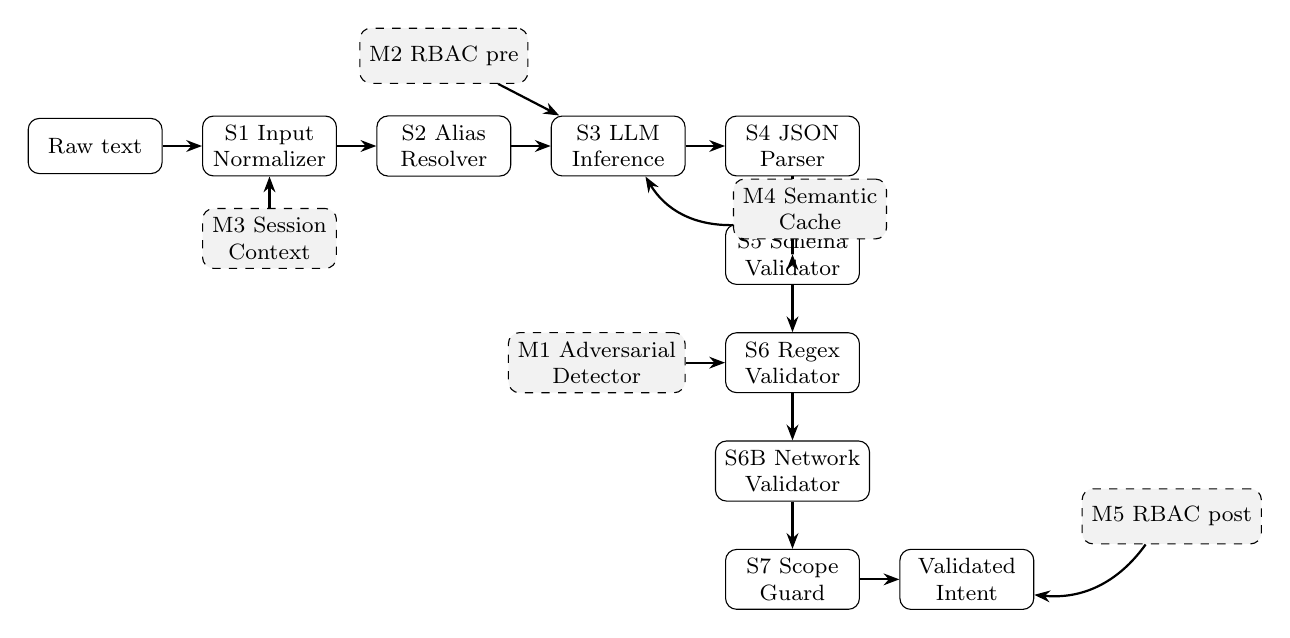
\begin{tikzpicture}[
  node distance=4mm and 5mm,
  stage/.style={draw, rectangle, rounded corners, minimum width=17mm, minimum height=7mm, align=center, font=\footnotesize},
  mid/.style={draw, rectangle, rounded corners, dashed, minimum width=17mm, minimum height=7mm, align=center, font=\footnotesize, fill=black!5},
  arr/.style={-{Stealth[length=2mm]}, thick}
]
\node[stage] (i) {Raw text};
\node[stage, right=of i] (s1) {S1 Input\\Normalizer};
\node[stage, right=of s1] (s2) {S2 Alias\\Resolver};
\node[stage, right=of s2] (s3) {S3 LLM\\Inference};
\node[stage, right=of s3] (s4) {S4 JSON\\Parser};
\node[stage, below=6mm of s4] (s5) {S5 Schema\\Validator};
\node[stage, below=6mm of s5] (s6) {S6 Regex\\Validator};
\node[stage, below=6mm of s6] (s6b) {S6B Network\\Validator};
\node[stage, below=6mm of s6b] (s7) {S7 Scope\\Guard};
\node[stage, right=of s7] (o) {Validated\\Intent};
\draw[arr] (i) -- (s1);
\draw[arr] (s1) -- (s2);
\draw[arr] (s2) -- (s3);
\draw[arr] (s3) -- (s4);
\draw[arr] (s4) |- (s5);
\draw[arr] (s5) -- (s6);
\draw[arr] (s6) -- (s6b);
\draw[arr] (s6b) -- (s7);
\draw[arr] (s7) -- (o);
\node[mid, left=of s6] (m1) {M1 Adversarial\\Detector};
\node[mid, above=4mm of s2] (m2) {M2 RBAC pre};
\node[mid, below=4mm of s1] (m3) {M3 Session\\Context};
\node[mid, right=6mm of s3, yshift=-8mm] (m4) {M4 Semantic\\Cache};
\node[mid, right=6mm of o, yshift=8mm] (m5) {M5 RBAC post};
\draw[arr] (m1) -- (s6);
\draw[arr] (m2) -- (s3);
\draw[arr] (m3) -- (s1);
\draw[arr] (m4) edge[bend left] (s3);
\draw[arr] (m5) edge[bend left] (o);
\end{tikzpicture}}
\caption{Guarded intent-recognition pipeline. Solid boxes run on every request; dashed middleware enforce security invariants and shortcut the core where possible.}
\label{fig:arch}
\end{figure}

\textbf{Core stages.} S1 normalizes casing, whitespace, and unicode. S2 resolves aliases (e.g., ``nmap -sS''~\cite{lyon2009nmap} $\rightarrow$ SCAN) against a catalog of 26 sub-intents spanning nine top-level intents (SCAN, EXPLOITATION, PASSWORD\_\-ATTACK, DIRECTORY\_\-BRUTE\-FORCE, CVE\-LOOKUP, RECON, PHISHING, NETWORK\-DEFENSE, MISC). S3 asks the LLM to emit a fixed JSON schema at temperature 0.4. S4 parses the response and fails fast on malformed JSON. S5 validates against the schema; S6 applies regex rules (host syntax, CIDR, port ranges). S6B, the network validator, resolves the target and checks it against the authorization policy and RFC~1918 private ranges~\cite{rfc1918}. S7, the scope guard, rejects requests whose target or technique falls outside the operator's declared scope. Only output that survives S5--S7 is returned; otherwise the stage-specific guard emits a classified error.

\textbf{Middleware.} M1 is the three-layer adversarial detector: a lexical layer assigns suspicion to prompt tokens (weights 0.8--1.0), a structural layer scores sentence topology and imperative-but-unclassifiable phrasing (0.3--0.9), and a scoring layer fuses both cumulatively; a cumulative score above 0.7 flags the request, and 0.95 auto-blocks without inference. M2/RBAC pre checks the caller's role before any inference is paid for; a \texttt{viewer} role fast-fails before S3. M3 maintains session context (user, role, target history). M4 is a semantic cache keyed on normalized embedding distance (Sentence-BERT~\cite{reimers2019sbert}): identical intents short-circuit the LLM entirely. M5 re-validates authorization on the final intent, so a single bypassed guard is not by itself sufficient to manufacture an authorized action.

\textbf{RBAC model.} Four roles (viewer, analyst, operator, admin) gate the nine intents. The three sensitive intents --- EXPLOITATION, PASSWORD\_ATTACK, DIRECTORY\_BRUTEFORCE --- require at least \texttt{operator}; EXPLOITATION covers offensive tooling drivers such as the Metasploit Framework~\cite{metasploit}. The default role is \texttt{analyst}; an unknown caller is downgraded to \texttt{viewer}. Enforcement occurs both pre-inference (M2, before cost is incurred) and post-validation (M5, on the final intent).

\textbf{Deployment properties.} The service runs headless, retrieves nothing at inference time (no RAG), and holds no secrets other than the model weights. Because there is no retrieval and no free-form output is ever rendered to a downstream shell, the two dominant remote attack classes --- indirect prompt injection via retrieved data~\cite{greshake2023indirect} and tool-injection via unfiltered text --- are structurally reduced to the narrower problem of classifying the single user utterance.

\textbf{Threat model.} Assets are the operator's security toolchain and system state. The trust boundary is the single device: no request leaves it, nothing is retrieved, and no output is rendered. The attacker controls the user utterance but not the device, prompts, policies, or model weights. Under this boundary the evaluated attack surfaces are direct adversarial utterances (handled by M1 and the RBAC matrix; 95.6\% of adversarial records caught) and authorization escalation (M2/M5). Indirect prompt injection via retrieved content and tool-injection via rendered text are structurally out of scope because neither channel exists; physical compromise of the device and backdoors embedded in the model weights are out of scope.

\textbf{\textcolor{nscblue}{Formal model.}} Let $\mathcal{X}$ be the utterance space, $\mathcal{Y}$ the nine-intent space, $\mathcal{C}$ the eight flaw classes, and $\mathcal{R}$ the role set. The decoder is a stochastic map $f:\mathcal{X}\to\mathcal{Z}$ producing observation $z\sim f(x)$; the deterministic guards are boolean predicates $g_5(z)$, $g_6(z)$, $g_{6B}(z,x)$, $g_7(x)$ over S5--S7, and the RBAC check $b:\mathcal{R}\times\mathcal{Y}\to\{0,1\}$. The guarded outcome is the decision
\begin{equation}
\Phi(x) = \begin{cases}
y\in\mathcal{Y}\ \text{accepted}, & G(z,x) \wedge b(\rho,y) \wedge \neg\, m_1(x),\\[2pt]
e\in\mathcal{C}\ \text{blocked}, & \text{otherwise},
\end{cases}
\label{eq:decision}
\end{equation}
with $G(z,x)=g_5\wedge g_6\wedge g_{6B}\wedge g_7$ and $\rho$ the caller role. The safety invariant the stack enforces is that every accepted output is schema-valid, network-authorized, in-scope, role-permitted, and non-adversarial:
\begin{equation}
\textsc{Accepted}(\Phi(x)) \;\Rightarrow\; \bigwedge\nolimits_{k\in\{S5,S6,S6B,S7,\mathrm{RBAC},M1\}} P_k(x).
\label{eq:invariant}
\end{equation}
The pipeline value (Exp1) is then precisely the gap in $\Pr\left[\bigwedge_k P_k\right]$ between raw $f$ and guarded $\Phi$; and a layer ablation (Exp3) estimates $\Pr[\mathrm{Accepted}]$ with each predicate $P_\ell$ removed --- the $\Delta$Catch column.

\section{METHODOLOGY}\label{sec:method}
\textbf{Setup.} All runs executed on an ASUS VivoBook X513EA (Intel Core i5-1135G7, 4 cores/8 threads, 24~GB DDR4, Windows 11) with Ollama in CPU-only mode. Backends are \texttt{qwen2.5-coder:7b} (4.7~GB) and \texttt{gemma4:e4b} (9.6~GB on disk), the build to which the \texttt{gemma4:latest} alias resolved at evaluation time. The exact Ollama version and per-model image digests as fetched are pinned in the evaluation manifest, which is the authoritative anchor for reproducing this study. No GPU is used; this reproduces the field deployment.

\textbf{Dataset.} Table~\ref{tab:dataset} summarizes the 900-record data set ($D$): 400 well-formed prompts (the $D^+$ set) and 500 flawed prompts ($D^-$) across eight categories, each with a gold intent label and a gold flaw label. Category sizes are deliberately non-uniform (24--100 records per class), reflecting per-category authoring feasibility rather than experimental design; per-class catch rates are therefore reported against each class's own size, and cross-category comparisons should be read with the differing denominators in mind.

\begin{table}[!t]
\centering
\caption{Data set composition ($N{=}900$). $D^+$ contains 400 well-formed prompts across nine intents; $D^-$ contains 500 flawed prompts.}
\label{tab:dataset}
\setlength{\tabcolsep}{4pt}
\small
\begin{tabular}{@{}lc@{}}
\toprule
\textbf{Category} & \textbf{Records} \\
\midrule
$D^+$ well-formed prompts & 400 \\
Adversarial injection & 100 \\
Out-of-scope target/technique & 90 \\
Ambiguous / under-specified & 30 \\
Contradictory request & 64 \\
Fabricated parameter & 64 \\
Fabricated CVE & 64 \\
Type mismatch (string vs.\ intent) & 64 \\
RBAC violation & 24 \\
\midrule
Total & 900 \\
\bottomrule
\end{tabular}
\end{table}

\textbf{\textcolor{nscteal}{Metrics.}} Let $y^\ast(x)$ and $c^\ast(x)$ denote the gold intent and flaw labels, $\hat{y}(x)$ the recognized intent, and $\hat{c}(x)$ the classified flaw. All three rates are reported as percentages:
\begin{align}
\mathrm{DAcc} &= \frac{1}{|D^+|}\sum_{x\in D^+}\mathbf{1}\!\big[\hat{y}(x)=y^\ast(x)\big]\times 100,\\
\mathrm{Catch} &= \frac{1}{|D^-|}\sum_{x\in D^-}\mathbf{1}\!\big[\hat{c}(x)=c^\ast(x)\big]\times 100,\\
\mathrm{FP} &= \frac{1}{|D^+|}\sum_{x\in D^+}\mathbf{1}\!\big[\text{a guard flags } x\big]\times 100.
\end{align}
DAcc and Catch are the two safety properties a copilot must hold simultaneously --- it must do the right thing (DAcc) and must not do the wrong thing (Catch) --- while FP measures how often a guard shadow-bans a legitimate operator.

\textbf{Experiments.}
\begin{itemize}
\item{\textbf{Exp1 (pipeline value).}} Compare raw single-shot LLM output against the full guarded pipeline on a 200-prompt stratified holdout (100 $D^+$, 100 $D^-$), per backend.
\item{\textbf{Exp2 (backend head-to-head).}} Fix the guardrail stack; compare Gemma vs.\ Qwen on the full holdout with identical prompts.
\item{\textbf{Exp3 (ablation).}} On the Qwen backend, re-run the full 900-record set once per disabled layer (scope guard off, RBAC off, network validator off, hallucination validator off, validation stack off, self-consistency off, semantic cache off), yielding eight configurations. The ``validation stack'' here is the entire deterministic validation stack (S5 schema, S6 regex, S6B network, S7 scope) disabled at once; it is a \emph{combined} ablation, not a single layer, and is reported because it bounds the stack's joint contribution.
\item{\textbf{Exp4 (per-class catch).}} Per-flaw-category catch rate on the Qwen backend.
\end{itemize}

\textbf{Implementation notes.} The self-consistency gate takes the decoding strategy of Wang \emph{et al.}~\cite{wang2023selfconsistency} from chain-of-thought sampling to classification agreement: it samples $k{=}3$ responses $\{z_i\}$ at temperature 0.6 and clusters them against the primary via embedding similarity. The agreement signal is
\begin{equation}
\alpha(x) = \frac{1}{\binom{k}{2}}\sum_{1\le i<j\le k}\mathbf{1}\!\big[d_{\mathrm{cos}}\big(\mathbf{e}(z_i),\mathbf{e}(z_j)\big)\le\theta_s\big],
\label{eq:agreement}
\end{equation}
where $\mathbf{e}(\cdot)$ is the Sentence-BERT embedding and $\theta_s$ the semantic threshold; raw single-sample $\alpha{=}1$. With two \emph{additional} samples, disagreement above $\theta_s$ demotes confidence and routes to the hallucination validator, which applies the six-class error taxonomy (impossible CVE, impossible parameter range, unverifiable value, contradictory fields, out-of-scope reference, unresolved type) and selects BLOCK, WARN, or ESCALATE accordingly. The full harness --- data, prompts, and evaluation scripts --- is versioned with the project source and regenerated by a single command.

\section{IMPLEMENTATION}
NeuroShell IRE is implemented as a modular Python service with a FastAPI surface and a clean internal split between the \texttt{core} (S1--S7), the \texttt{guards} (M1--M5), and the \texttt{llm} adapter. Backend swap is a single configuration change; both Ollama models expose the same chat API. The schema validator uses a hand-written recursive validator (kept dependency-light for a cold-start device) rather than a heavyweight runtime. The adapter enforces a per-stage timeout so that an unresponsive model cannot stall the pipeline. Deterministic guards (S5, S6, S6B, S7) and the pre-inference RBAC check run with zero LLM dependency, so the \texttt{viewer} path is a pure function of the request that costs milliseconds.

The test suite comprises 482 automated tests (434 unit, 48 asynchronous integration) measured on 2026-08-26, covering every guard path, RBAC matrix cells, cache hit/miss paths, and the six-class hallucination policy. The dataset and harness are versioned with the source; evaluation is a single reproducible command that regenerates all tables in this paper.

\section{EVALUATION AND RESULTS}\label{sec:results}
\textbf{Exp1 --- pipeline value.} Raw single-shot output made no structured intent available in 100\% of flawed cases (catch $0\%$) and misclassified 22\% (Gemma) and 31\% (Qwen) of well-formed prompts. Adding the guarded pipeline raised DAcc from 78 to 86\% (Gemma) and 69 to 82\% (Qwen), raised catch from $0\%$ to 72\% (Gemma) and 64\% (Qwen), and cut the FP rate from 32\% to 14\% (Gemma) and from 31\% to 15\% (Qwen), i.e.,\ the number of well-formed prompts a guard erroneously flags. All FP reductions are conservative well-formed ``over-blocks,'' never a dangerous misclassification toward a privileged intent. The improvement is largest for catch rate because every flawed category is caught by at least one deterministic guard, whereas raw output is never flagged.

\begin{table}[!t]
\centering
\caption{Exp1: raw LLM output vs.\ guarded pipeline (200-prompt holdout).}
\label{tab:exp1}
\setlength{\tabcolsep}{4pt}
\small
\begin{tabular}{@{}lcccc@{}}
\toprule
\textbf{Config} & \textbf{DAcc\%} & \textbf{Catch\%} & \textbf{FP\%} \\
\midrule
Gemma raw         & 78 & 0  & 32 \\
Gemma guarded     & 86 & 72 & 14 \\
Qwen raw          & 69 & 0  & 31 \\
Qwen guarded      & 82 & 64 & 15 \\
\bottomrule
\end{tabular}
\end{table}

\textbf{Exp2 --- backend head-to-head.} Under identical guardrails, Gemma leads on DAcc (86 vs.\ 82) and catch (72 vs.\ 64), with similar FP (14 vs.\ 15). The guarded architecture reduces backend sensitivity: while raw Gemma already outperformed raw Qwen by 9 points, the pipeline closes the DAcc gap to 4 points and holds catch within 8 points, indicating that the deterministic layers dominate residual accuracy for well-formed inputs.

\begin{table}[!t]
\centering
\caption{Exp2: identical guardrail stack for both backends (200-prompt holdout).}
\label{tab:exp2}
\setlength{\tabcolsep}{4pt}
\small
\begin{tabular}{@{}lccc@{}}
\toprule
\textbf{Backend} & \textbf{DAcc\%} & \textbf{Catch\%} & \textbf{FP\%} \\
\midrule
Gemma (guarded) & 86 & 72 & 14 \\
Qwen (guarded)  & 82 & 64 & 15 \\
\bottomrule
\end{tabular}
\end{table}

\textbf{Exp3 --- ablation.} Table~\ref{tab:exp3} shows the effect of removing each layer on the full 900-record set with the Qwen backend. The marginal contribution of a layer $\ell$ is the difference against the baseline pipeline $\Pi$, $\Delta_{\mathrm{catch}}(\ell) = \mathrm{Catch}(\Pi) - \mathrm{Catch}(\Pi\setminus\ell)$, which is the rightmost column. The validation stack as a whole is the dominant safety contributor: disabling it drops catch from 84 to 41 (${-}43$~points) and DAcc from 73.5 to 64.0. Its FP rate also falls sharply, from 34\% to 13\%, because with S5--S7 disabled only the adversarial detector (M1) and pre-inference RBAC remain able to flag a well-formed prompt --- and they do so rarely. Within the stack, the hallucination validator is the single largest catch contributor (${-}22$~points), and the scope guard the largest accuracy contributor (${-}9.5$~points). Removing RBAC \emph{increases} DAcc by 1.0 point while dropping catch by 20, and cuts the FP rate from 34\% to 22\%, revealing a benign-versus-safe tension: RBAC refuses legitimate-looking requests that fall outside the caller's role --- a deliberate over-block trade accepted for safety. The network validator contributes little at the aggregate level (${-}5.5$ DAcc, ${-}2$ catch) because its effect concentrates on the few records whose only detectable flaw is an invalid or policy-violating target. The self-consistency and semantic-cache layers both reduce catch when removed (${-}4$ and ${-}5$) while also raising the FP rate (${+}11$ and ${+}13$~points), confirming that the cache improves determinism as well as latency.

\begin{table}[!t]
\centering
\caption{Exp3: ablation on the full dataset (Qwen, $N{=}900$).}
\label{tab:exp3}
\setlength{\tabcolsep}{4pt}
\small
\begin{tabular}{@{}lcccc@{}}
\toprule
\textbf{Configuration} & \textbf{DAcc\%} & \textbf{Catch\%} & \textbf{FP\%} & $\Delta$Catch \\
\midrule
Full pipeline (baseline) & 73.5 & 84 & 34 & --- \\
No scope guard           & 64.0 & 73 & 44 & $-11$ \\
No RBAC guard            & 74.5 & 64 & 22 & $-20$ \\
No network validator     & 68.0 & 82 & 44 & $-2$ \\
No halluc. validator     & 65.4 & 62 & 44 & $-22$ \\
No validation stack      & 64.0 & 41 & 13 & $-43$ \\
No self-consistency      & 67.5 & 80 & 45 & $-4$ \\
No semantic cache        & 66.0 & 79 & 47 & $-5$ \\
\bottomrule
\end{tabular}
\end{table}

\textbf{Exp4 --- per-class catch.} On a dedicated 250-record deep-dive set of flawed prompts (100 from $D^-$ plus 150 newly generated, Qwen backend), catch is strongest exactly where deterministic rules exist. Adversarial injection is caught at 95.6\% (43/45) by M1's lexical/structural layers, and RBAC violations at 100\% (12/12) by the deterministic pre-inference role check (a small sample --- n${=}$12 --- so this is not a tight bound, though the check is rule-based rather than model-sampled). Fabricated parameters (87.5\%, 28/32) and type mismatches (81.3\%, 26/32) are caught by the S5--S6 syntactic rules; fabricated CVEs (78.1\%, 25/32) by the hallucination validator's offline CVE grounding. The residual weak classes are the semantic ones --- contradictory requests (59.4\%, 19/32), out-of-scope (46.7\%, 21/45), and ambiguous (40\%, 8/20) --- where no deterministic signal exists and the system must rely on the self-consistency gate and the LLM's own agreement. These three classes are also the largest share of the full dataset's flaws: under the 900-record denominators of Table~\ref{tab:dataset} they sum to 184 of the 500 flawed records (90 out-of-scope, 64 contradictory, 30 ambiguous), versus 45, 32, and 20 in the 250-record deep-dive set above --- so per-class reporting against each denominator, not an aggregate catch number, is the appropriate basis for a security claim.

\textbf{Latency.} On CPU-only hardware, end-to-end p50 is $\approx$16.5~s and p95 $\approx$70.9~s for cache-miss requests; disabling self-consistency lowers p50 to $\approx$13.4~s (the two extra samples add roughly 3~s), and the ablation shows it is the largest latency component. Semantic-cache hits resolve in $\approx$44~ms, a $\approx$375$\times$ speedup, i.e.,\ $\tfrac{\mathbb{E}[t\mid\mathrm{miss}]}{\mathbb{E}[t\mid\mathrm{hit}]}\approx 375$, which makes repeated or scripted intents viable offline. These figures bound the practical constraint behind the design: any guard that adds a \emph{third} LLM call was rejected because it would push p95 beyond two minutes on this class of hardware.

\section{DISCUSSION}
Our results answer the three research questions directly.

\textbf{RQ1: pipeline value.} The guarded pipeline is the difference between unusable and usable output: it turns a hallucinating, injection-prone free-form generator into a structured classifier whose output must pass deterministic checks on the well-formed side, and it catches most flawed inputs before they reach a tool. The catch-rate leap (0$\rightarrow$64--72 on the holdout, up to 84 on the 900-record ablation set) is the key result; raw LLM output contains no machine-checkable safety property at all.

\textbf{RQ2: layer contribution.} Hallucination validation and the full validation stack dominate catch; the scope guard dominates accuracy; RBAC trades a point of DAcc for 20 points of catch. Network validation is class-critical but aggregate-invisible \emph{without} Exp4, which is why per-class reporting is essential for security claims. Crucially, layers interact constructively: removing RBAC damages catch more than removing the network validator, despite RBAC's small DAcc contribution, because the pre-inference fast-fail prevents a class of out-of-role requests from ever being misclassified as authorized.

\textbf{RQ3: generality.} The guardrails hold for both backends with the same ordering of effects; the deterministic stages compress, but do not erase, raw-model quality differences. This supports treating the decoder as a swappable component of a \emph{guarded system} rather than the security boundary itself.

\textbf{Threat model boundaries.} The design converts a fully open problem --- making an LLM trustworthy --- into a closed one: classify a single user utterance under known policy. This is defensible \emph{because} the system retrieves nothing and renders nothing; the standard indirect-injection and tool-injection channels~\cite{greshake2023indirect,owasp2025} are curtailed at the boundary. What remains is direct adversarial utterance, which M1 and the RBAC matrix address, and measurement shows 95.6\% catch on adversarial records.

\section{LIMITATIONS AND THREATS TO VALIDITY}
\textbf{Internal validity.} Exp3's baseline was measured on the 900-record set while Exp1/Exp2 used a 200-prompt stratified holdout; the DAcc values (73.5 vs.\ 82) therefore differ across datasets and must not be compared directly. The dataset is synthetic --- authored, not sampled from production traffic --- so real speech patterns may shift class difficulty. One layer (semantic cache) changes not only latency but also determinism, meaning its ablation conflates a performance effect with a correctness effect; the $-5$ catch figure may overstate the layer's purely semantic contribution. Because the Exp3 ``no validation stack'' row disables S5--S7 as one condition, its ${-}43$ catch shift is a \emph{combined} ablation and does not isolate any single stage. RBAC's perfect Exp4 catch rests on n${=}$12 records and reflects a deterministic role lookup, not a general capability. Finally, backend identity (tag, quantization, on-disk size) and the exact Ollama version are pinned in the evaluation manifest but were not independently re-verified against public model cards.

\textbf{External validity.} Experiments use two Ollama-hosted, instruction-tuned 7--9~B models on one laptop. Larger or differently-aligned models may exhibit different failure modes, and cloud models with higher base accuracy may leave less headroom for validation to add. Every experiment is a single run without seed variance or confidence intervals: the pipeline is stochastic (temperature-0.4 decoding, non-deterministic scheduler), so the reported figures are point estimates of bimodal latencies and near-certain class accuracies, not bounds; backend- and seed-averaged reruns with interval reporting are the first planned extension. The hallucination validator's CVE grounding is a hand-curated 20-entry list; identifiers outside it are treated as plausible zero-days rather than auto-blocked, a deliberately conservative policy where a snapshot refreshed from the National Vulnerability Database~\cite{nistnvd} and scored with EPSS~\cite{firstepss} would tighten coverage at the cost of the offline boundary. \textbf{Construct validity.} DAcc and catch are our constructs for ``right'' and ``not wrong''; a user may disagree about borderline classes (contradictory vs.\ ambiguous), which contributes label noise to the 40--59\% classes. \textbf{Threats unique to offline deployment.} We found that offline CPU-only models produce a distinct failure profile --- verbose JSON with embedded commentary, and higher per-call variance --- that the deterministic stages must absorb; a pipeline tuned on API-grade models would miss these patterns. Finally, RBAC and network policy are evaluations of \emph{configuration}, so the measured catch reflects the test policy set, not an absolute security guarantee for other operators.

\section{CONCLUSION}
We presented NeuroShell IRE, a guarded intent-recognition engine that makes a small, offline, CPU-only LLM reliable enough to gate an operational security copilot under the evaluated threat model. On a 900-record data set spanning eight flaw classes and a per-layer ablation across eight configurations, the pipeline raises catch from $0\%$ to 64--72\% on the stratified holdout and 84\% on the 900-record ablation set, raises accuracy from 69--78\% to 82--86\%, and isolates the dominant safety layer (hallucination validation, ${-}22$ points of catch if removed). The results hold across two distinct backends, showing that deterministic guardrailing, not model choice, is the load-bearing security property --- provided the boundary is closed (no retrieval, no free-form rendering). Residual weakness is concentrated in purely semantic flaw classes, pointing to better need for unsupervised agreement signals and per-operator policy learning as the next steps.

\begin{thebibliography}{18}
\bibitem{deng2024pentestgpt} G. Deng et al., ``PentestGPT: Evaluating and harnessing large language models for automated penetration testing,'' in \emph{Proc. 33rd USENIX Security Symp. (USENIX Security)}, Philadelphia, PA, USA, 2024, pp. 847--864.
\bibitem{happe2023pwned} A. Happe and J. Cito, ``Getting pwn'd by AI: Penetration testing with large language models,'' in \emph{Proc. 31st ACM Joint Eur. Softw. Eng. Conf. and Symp. on Found. of Softw. Eng. (ESEC/FSE)}, San Francisco, CA, USA, 2023, pp. 2082--2086.
\bibitem{greshake2023indirect} K. Greshake, S. Abdelnabi, S. Mishra, C. Endres, T. Holz, and M. Fritz, ``Not what you've signed up for: Compromising real-world LLM-integrated applications with indirect prompt injection,'' in \emph{Proc. 16th ACM Workshop Artif. Intell. and Security (AISec)}, Copenhagen, Denmark, 2023, pp. 79--90.
\bibitem{liu2023promptinjection} Y. Liu, Y. Jia, R. Geng, J. Jia, and N. Z. Gong, ``Prompt injection attacks and defenses in LLM-integrated applications,'' arXiv:2310.12815, 2023.
\bibitem{kang2024dualuse} D. Kang, X. Li, I. Stoica, C. Guestrin, M. Zaharia, and T. Hashimoto, ``Exploiting programmatic behavior of LLMs: Dual-use through standard security attacks,'' in \emph{Proc. IEEE Security and Privacy Workshops (SPW)}, San Francisco, CA, USA, 2024, pp. 132--143.
\bibitem{owasp2025} OWASP Foundation, ``OWASP Top 10 for Large Language Model Applications, 2025,'' genai.owasp.org, 2025. [Online]. Available: \url{https://genai.owasp.org/}
\bibitem{ji2023hallucination} Z. Ji et al., ``Survey of hallucination in natural language generation,'' \emph{ACM Comput. Surv.}, vol. 55, no. 12, pp. 1--38, 2023.
\bibitem{manakul2023selfcheckgpt} P. Manakul, A. Liusie, and M. J. F. Gales, ``SelfCheckGPT: Zero-resource black-box hallucination detection for generative large language models,'' in \emph{Proc. EMNLP}, Singapore, 2023, pp. 9004--9017.
\bibitem{kuhn2023semantic} L. Kuhn, Y. Gal, and S. Farquhar, ``Semantic uncertainty: Linguistic invariances for uncertainty estimation in natural language generation,'' in \emph{Proc. ICLR}, Kigali, Rwanda, 2023.
\bibitem{farquhar2024semantic} S. Farquhar, J. Kossen, L. Kuhn, and Y. Gal, ``Detecting hallucinations in large language models using semantic entropy,'' \emph{Nature}, vol. 630, no. 8017, pp. 625--630, 2024.
\bibitem{wang2023selfconsistency} X. Wang, J. Wei, D. Schuurmans, Q. Le, E. H. Chi, S. Narang, A. Chowdhery, and D. Zhou, ``Self-consistency improves chain of thought reasoning in language models,'' in \emph{Proc. ICLR}, Kigali, Rwanda, 2023.
\bibitem{lewis2020rag} P. Lewis, E. Perez, A. Piktus, F. Petroni, V. Karpukhin, N. Goyal, H. K\"uttler, M. Lewis, W. Yih, T. Rockt\"aschel, S. Riedel, and D. Kiela, ``Retrieval-augmented generation for knowledge-intensive NLP tasks,'' in \emph{Proc. NeurIPS}, Vancouver, Canada, 2020, pp. 9459--9474.
\bibitem{reimers2019sbert} N. Reimers and I. Gurevych, ``Sentence-BERT: Sentence embeddings using Siamese BERT-networks,'' in \emph{Proc. EMNLP-IJCNLP}, Hong Kong, 2019, pp. 3982--3992.
\bibitem{rfc1918} Y. Rekhter, B. Moskowitz, D. Karrenberg, G. de Groot, and E. Lear, ``Address allocation for private internets,'' IETF, RFC 1918, 1996. [Online]. Available: \url{https://www.rfc-editor.org/rfc/rfc1918}
\bibitem{nistnvd} National Institute of Standards and Technology, ``National Vulnerability Database (NVD),'' nvd.nist.gov. [Online]. Available: \url{https://nvd.nist.gov/}
\bibitem{firstepss} FIRST.org, ``Exploit Prediction Scoring System (EPSS),'' first.org. [Online]. Available: \url{https://www.first.org/epss/}
\bibitem{lyon2009nmap} G. F. Lyon, \emph{Nmap Network Scanning}. Sunnyvale, CA, USA: Insecure.Com LLC, 2009.
\bibitem{metasploit} Rapid7, ``Metasploit Framework,'' rapid7.com. [Online]. Available: \url{https://www.metasploit.com/}
\end{thebibliography}

\end{document}